\begin{frame}
\end{frame}

\begin{frame}

\section{Density Estimation: What and Why?}
\notesonly{
We observe data. 
This data is generated by some unknown probability distribution. Each observation is a sample from this distrubtion.
When we talk about density estimation, we are talking about recovering the underlying probability density function that produced te observed samples.
}

\question{Why do we care about estimating densities? What can we do with an estimated density?}

\begin{itemize}
\item data exploration
\item visualization (for 1D and 2D data)
\item deduce moments (mean, variance, \ldots)
\item describe the data in compact form (e.g. this data follows a Gaussian with mean $\mu$ and covariance $\vec \Sigma$)
\item generate new data
\item unsupervised anomaly detection
\end{itemize}

\end{frame}

\begin{frame}

\underline{Density Estimation: How?}

2 strategies:

\begin{enumerate}[(A)]
\item \textbf{parametric} methods:
\\ We assume that the data follows some class of distribution and we estimate its paramters (e.g. fit a Gaussian around this data)
\item \textbf{non-parametric}\footnote{non-parametric does not means it is void of paramters. 
It is just that the parameters do not directly correspond to the classical parameters of densities such as mean and variance.} methods: 
data-driven. Estimate the density with as few assumptions as possible (e.g. Kernel\footnote{Not tied to Mercer Kernels like in Kernel PCA. A kernel is just some non-negative function.} density estimation)
\end{enumerate}

\end{frame}

Many people habe already encountered density estimation in the form of histograms.

\begin{frame}
\end{frame}

\begin{frame}

\begin{figure}[ht]
     \centering
     \savebox{\imagebox}{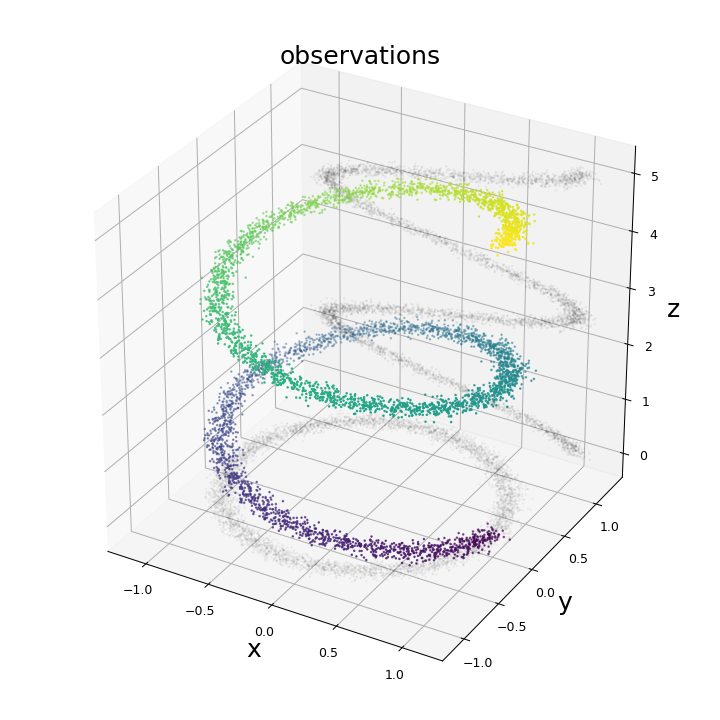
\includegraphics[width=0.4\textwidth]{img/spiral_data.png}}%
     \begin{subfigure}[t]{0.4\textwidth}
         \centering
         \usebox{\imagebox}% Place largest image
         \caption{original observations $\vec x$}
         \label{fig:spiral_data}
     \end{subfigure}
     \hfill
     \begin{subfigure}[t]{0.35\textwidth}
         \centering
         \raisebox{\dimexpr.5\ht\imagebox-.5\height}{% Raise smaller image into place
         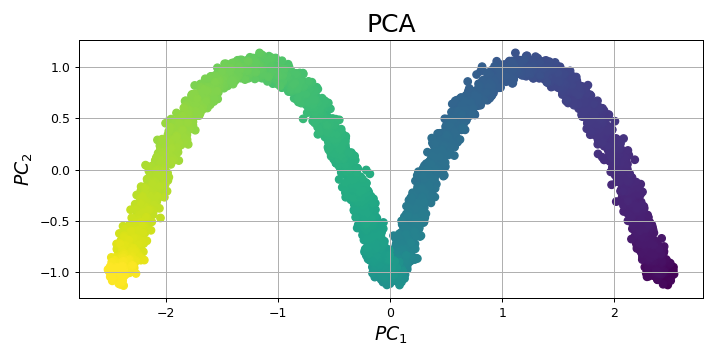
\includegraphics[width=\textwidth]{img/spiral_pca.png}
         }
         \caption{projection onto the first 2 PCs}
         \label{fig:spiral_pca}
     \end{subfigure}
     \caption{Dimensionality reduction of ``spiral data''. Points are colored according to their index in the dataset.}
	 \label{fig:spiral}
\end{figure}

\end{frame}

